\documentclass[11pt,a4paper]{article}

\usepackage[utf8]{inputenc}
\usepackage[spanish]{babel}
\usepackage{amsmath}
\usepackage{amsfonts}
\usepackage{amssymb}
\usepackage{makeidx}
\usepackage{graphicx}
\usepackage{lmodern}
\usepackage{kpfonts}
\usepackage{wrapfig}
\usepackage{caption}
\usepackage{subcaption}
\usepackage{booktabs}
\usepackage[nottoc,numbib]{tocbibind} %agrega la bibliografia al índice.
\usepackage[font={small,it}]{caption}
%\usepackage{fourier}
\usepackage[left=2cm,right=2cm,top=2cm,bottom=2cm,headheight=13.6pt]{geometry}
\usepackage{fancyhdr}
\usepackage{multirow}
\pagestyle{fancy}


%Para los gráficos en general, con las tablas...¡Ja!, arreglate.
%\begin{figure}[h!]
%\centering
%\includegraphics[width=0.7\textwidth]{} %nombre de la imagen, incluirla en el mismo directorio que este archivo.
%\caption*{} %rótulo, el asterico elimina la numeración automática. 
%\label{fig:} % para luego referirse con \ref{fig:}
%\end{figure}


\begin{document}


%%%%%%%%%%%%%%%%%%%%%%%%%%%%%%%%%%%%%%%%%%%%%%%%%%%%%%%%%%%%%%%%%%%%%%%%%%%%%%%%%%%%%%%%%%%%%%%%%%%%%%%%%%%%%%%%%%%%%%%%%%%%%%%%%
% 	TÍTULO
%%%%%%%%%%%%%%%%%%%%%%%%%%%%%%%%%%%%%%%%%%%%%%%%%%%%%%%%%%%%%%%%%%%%%%%%%%%%%%%%%%%%%%%%%%%%%%%%%%%%%%%%%%%%%%%%%%%%%%%%%%%%%%%%%

%%%%%%%%%%%%%%%%%%%%%%%%%%%%%%%%%%%%%%%%%
% University Assignment Title Page 
% LaTeX Template
% Version 1.0 (27/12/12)
%
% This template has been downloaded from:
% http://www.LaTeXTemplates.com
%
% Original author:
% WikiBooks (http://en.wikibooks.org/wiki/LaTeX/Title_Creation)
%
% License:
% CC BY-NC-SA 3.0 (http://creativecommons.org/licenses/by-nc-sa/3.0/)
% 
% Instructions for using this template:
% This title page is capable of being compiled as is. This is not useful for 
% including it in another document. To do this, you have two options: 
%
% 1) Copy/paste everything between \begin{document} and \end{document} 
% starting at \begin{titlepage} and paste this into another LaTeX file where you 
% want your title page.
% OR
% 2) Remove everything outside the \begin{titlepage} and \end{titlepage} and 
% move this file to the same directory as the LaTeX file you wish to add it to. 
% Then add \input{./title_page_1.tex} to your LaTeX file where you want your
% title page.
%
%%%%%%%%%%%%%%%%%%%%%%%%%%%%%%%%%%%%%%%%%

%----------------------------------------------------------------------------------------
%	PACKAGES AND OTHER DOCUMENT CONFIGURATIONS
%----------------------------------------------------------------------------------------

%\documentclass[12pt]{article}
%\usepackage[utf8]{inputenc}
%\usepackage[spanish]{babel}
%\begin{document}

\begin{titlepage}

\newcommand{\HRule}{\rule{\linewidth}{0.5mm}} % Defines a new command for the horizontal lines, change thickness here

\center % Center everything on the page
 
%----------------------------------------------------------------------------------------
%	HEADING SECTIONS
%----------------------------------------------------------------------------------------

\textsc{\Huge Universidad de Buenos Aires}\\[0.5cm]
\textsc{\LARGE Facultad de Ciencias Exactas y Naturales}\\[0.5cm] % Name of your university/college
\textsc{\Large Departamento de Física}\\[0.25cm] % Major heading such as course name

\begin{figure}[h]
  \centering
  
\includegraphics[scale=0.15]{Logo_DF}
  \\[0.5cm]
\end{figure}

\textsc{\large Laboratorio 3}\\[0.25cm] % Minor heading such as course title

%----------------------------------------------------------------------------------------
%	TITLE SECTION
%----------------------------------------------------------------------------------------

\HRule \\[0.4cm]
{ \huge \bfseries Transitorio y tiempo caracteristico de circuitos}\\[0.2cm] % Title of your document
\HRule \\[1cm]
 
%----------------------------------------------------------------------------------------
%	AUTHOR SECTION
%----------------------------------------------------------------------------------------

\begin{minipage}{0.4\textwidth}
\begin{center} \large
\emph{Autores:}\\
\textsc{Andreu}, Gonzalo\\ % Your name
\textsc{Malpartida}, Bryan\\ % Your name
\textsc{Pugliese}, Facundo\\ % Your name


\end{center}
\end{minipage}
~ \\[1.25cm]
%\begin{minipage}{0.4\textwidth}
%\begin{flushright} \large
%\emph{Supervisor:} \\
%Dr. James \textsc{Smith} % Supervisor's Name
%\end{flushright}
%\end{minipage}\\[4cm]

% If you don't want a supervisor, uncomment the two lines below and remove the section above
%\Large \emph{Author:}\\
%John \textsc{Smith}\\[3cm] % Your name

%----------------------------------------------------------------------------------------
%	DATE SECTION
%----------------------------------------------------------------------------------------

%\vspace{\fill}


{\large 17 de Febrero de 2016}\\[1.75cm] % Date, change the \today to a set date if you want to be precise

%----------------------------------------------------------------------------------------
%	SUMMARY SECTION: No más de 15 renglones, no te zarpes
%----------------------------------------------------------------------------------------

\begin{center}
\large{\textbf{Resumen}}

\small{El objetivo del siguiente trabajo fue caracterizar circuitos RC, RL y RCL. 

Para los dos primeros casos, los circuitos RC y RL, se buscó determinar el tiempos característico de cada uno variando los parámetros de cada sistema. Ademas de poder observar los fenómenos particulares en estos sistemas, como la carga y descarga del capacitor y la disminución de la corriente debido a la inductancia, utilizando una fuente de alimentación que emitía señales cuadradas y osciloscopio como instrumento de medición.

Por otro lado, el estudio del circuito RCL se centró en la observación de los comportamientos que tiene el mismo para distintos parámetros del sistema. Para ellos se obtenían teóricamente los valores necesarios de cada parámetro para luego $settear$ los elementos del circuito y comprobar que la evolución del sistema cumpliese el modelo teórico. Dichas observaciones se obtuvieron nuevamente utilizando una fuente de señal cuadrada y un osciloscopio.

Finalmente, el método resulto eficiente a la hora de comprobar las ecuaciones referidas al circuito RC y, en menor medida, al circuito RL. En el caso del circuito RCL, pudieron analizarse los casos extremos de comportamiento, pero no el comportamiento borde debido a lo fino del mismo.} % ACA VA EL RESUMEN

\end{center}


%----------------------------------------------------------------------------------------
%	LOGO SECTION
%----------------------------------------------------------------------------------------

%\includegraphics{Logo}\\[1cm] % Include a department/university logo - this will require the graphicx package
 
%----------------------------------------------------------------------------------------

\vfill % Fill the rest of the page with whitespace

\end{titlepage}
%\end{document} %incluir en el mismo directorio que este archivo. Equivalente a un copiar-pegar, nada de andar diciendo \begin{document} en la portada. Dejar el nombre de Caratula a la caratula.

%%%%%%%%%%%%%%%%%%%%%%%%%%%%%%%%%%%%%%%%%%%%%%%%%%%%%%%%%%%%%%%%%%%%%%%%%%%%%%%%%%%%%%%%%%%%%%%%%%%%%%%%%%%%%%%%%%%%%%%%%%%%%%%%%
% 	ENCABEZADO Y PIE DE PÁGINA.
%%%%%%%%%%%%%%%%%%%%%%%%%%%%%%%%%%%%%%%%%%%%%%%%%%%%%%%%%%%%%%%%%%%%%%%%%%%%%%%%%%%%%%%%%%%%%%%%%%%%%%%%%%%%%%%%%%%%%%%%%%%%%%%%%

\lhead{}
\chead{}
\rhead{Laboratorio 3}
\lfoot{}
\cfoot{}
\rfoot{\thepage}
\renewcommand{\headrulewidth}{1pt}
\renewcommand{\footrulewidth}{1pt}


%%%%%%%%%%%%%%%%%%%%%%%%%%%%%%%%%%%%%%%%%%%%%%%%%%%%%%%%%%%%%%%%%%%%%%%%%%%%%%%%%%%%%%%%%%%%%%%%%%%%%%%%%%%%%%%%%%%%%%%%%%%%%%%
% Página en blanco. Cita, agradecimiento, dedicación, lo que sea pero que sea algo.
%%%%%%%%%%%%%%%%%%%%%%%%%%%%%%%%%%%%%%%%%%%%%%%%%%%%%%%%%%%%%%%%%%%%%%%%%%%%%%%%%%%%%%%%%%%%%%%%%%%%%%%%%%%%%%%%%%%%%%%%%%%%%%%


%%%%%%%%%%%%%%%%%%%%%%%%%%%%%%%%%%%%%%%%%%%%%%%%%%%%%%%%%%%%%%%%%%%%%%%%%%%%%%%%%%%%%%%%%%%%%%%%%%%%%%%%%%%%%%%%%%%%%%%%%%%%%%%%%
% 	ÍNDICE
%%%%%%%%%%%%%%%%%%%%%%%%%%%%%%%%%%%%%%%%%%%%%%%%%%%%%%%%%%%%%%%%%%%%%%%%%%%%%%%%%%%%%%%%%%%%%%%%%%%%%%%%%%%%%%%%%%%%%%%%%%%%%%%%%

%\tableofcontents %compilar dos o tres veces para verlo bien. ¡Todo un índice en unas cuantas letras!
%\newpage

%%%%%%%%%%%%%%%%%%%%%%%%%%%%%%%%%%%%%%%%%%%%%%%%%%%%%%%%%%%%%%%%%%%%%%%%%%%%%%%%%%%%%%%%%%%%%%%%%%%%%%%%%%%%%%%%%%%%%%%%%%%%%%%
% 1. RESUMEN
%%%%%%%%%%%%%%%%%%%%%%%%%%%%%%%%%%%%%%%%%%%%%%%%%%%%%%%%%%%%%%%%%%%%%%%%%%%%%%%%%%%%%%%%%%%%%%%%%%%%%%%%%%%%%%%%%%%%%%%%%%%%%%%

%\section{Resumen}
%\label{sec:resumen}



%%%%%%%%%%%%%%%%%%%%%%%%%%%%%%%%%%%%%%%%%%%%%%%%%%%%%%%%%%%%%%%%%%%%%%%%%%%%%%%%%%%%%%%%%%%%%%%%%%%%%%%%%%%%%%%%%%%%%%%%%%%%%%%
% 2. INTRODUCCIÓN: ecuaciones aquí, luego se las cita.
%%%%%%%%%%%%%%%%%%%%%%%%%%%%%%%%%%%%%%%%%%%%%%%%%%%%%%%%%%%%%%%%%%%%%%%%%%%%%%%%%%%%%%%%%%%%%%%%%%%%%%%%%%%%%%%%%%%%%%%%%%%%%%%

\section{Introducción}\label{sec:intro}
Este trabajo se centra alrededor del analisis de \textit{señales}. Una \textit{señal} es una diferencia de potencial $S(t)$ que se genera en alguna sección del circuito. En su forma más general, se puede definir una señal $S(t) = V_o.f(t)$ donde $V_o$ es un voltaje constante que representa la \textit{amplitud} y $f(t)$ es una función del tiempo que define el \textit{tipo de señal} y es la que define el comportamiento del circuito. Para un circuito compuesto por resistencias $R$, capacitancias $C$ e inductancias $L$, este comportamiento puede ser muy complicado de predecir teóricamente. Sin embargo, para una señal del tipo $V(t) = V_o.cos(\omega t)$ el comportamiento está ampliamente estudiado y resulta sencillo de predecir. 

Es aquí donde entra en juego la \textit{Serie de Fourier}, que consiste en escribir una función períodica $f(t)$ como una serie de senos y cosenos pesados por coeficientes $a_n$ y $b_n$ según. Funciones que no sean períodicas pero que estén definidas en un intervalo finito $[-\tau;\tau]$ también puede expandirse de forma períodica. Si $2\tau$ es el período (o la longitud del intervalo) de la funcion $f(t)$, se tiene que

\begin{equation}
f(t) = \frac{a_o}{2} + \Sigma_{n=1}^{\infty} a_n.cos(\frac{n\pi}{\tau}t) + b_n.sin(\frac{n\pi}{\tau}t) = \frac{a_o}{2} + \Sigma_{n=1}^{\infty} \alpha_n.cos(\frac{n\pi}{\tau}t+\phi_n)
\label{eq:fourier}
\end{equation}

donde 

\begin{equation}
\begin{split}
a_n = \frac{1}{\tau}\int_{-\tau}^{\tau}f(t).cos(\frac{n\pi}{\tau}t)dt\\
b_n = \frac{1}{\tau}\int_{-\tau}^{\tau}f(t).sin(\frac{n\pi}{\tau}t)dt\\
\alpha_n = \sqrt{a_n^2+b_n^2}\\
\phi_n = -arctan(\frac{b_n}{a_n})
\end{split}
\label{eq:coefs}
\end{equation}

Entonces resulta posible considerar a toda señal $S(t)$ como una suma de infinitas señales sinusoidales y gracias a la linealidad de los componentes $R$, $C$ y $L$, el comportamiento será igual al comportamiento de la suma. Es más, considerando que vale $a_n \rightarrow 0$ y $b_n \rightarrow 0$ para $n \rightarrow \infty$, cada término de la sumatoria tendrá menos peso que los anteriores. Por lo tanto, es posible estimar el comportamiento aproximado del circuito como si la señal fuera una suma finita de sinusoides. Para una función $f(t)\in C^k$, cuanto mayor suave sea $k$, más rápido será este decaimiento y menos términos de la serie se necesitarán para aproximar el comportamiento. Bajo esta idea, si fuera posible filtrar una única frecuencia $\omega_n = \frac{n\pi}{\tau}$, se obtendría una señal de salida sinusoidal cuya amplitud sería $\alpha_n$. 

Este filtro puede ser un circuito RLC resonante, el cual consiste en una fuente $V(t) = V_o.cos(\omega t)$, un capacitor $C$, una inductancia $L$ (de resistencia interna $R_L$) y una resistencia $R$ conectados en serie. Si se mide la amplitud de la caida de potencial sobre la resistencia $R$ resulta de la forma $V_R = V_o\frac{R)}{|Z|}$ donde $Z = (R+R_L)+i(\omega.L-\frac{1}{\omega C})$. Definiendo la \textit{transmisión} $T(\omega) = \frac{V_R}{V_o}$ resulta $T(\omega) = \frac{R}{|Z|}$ cuyo máximo se encuentra en $\omega_o = \frac{1}{\sqrt{LC}}$ tal que $T_{max} = T(\omega_o) = \frac{R}{R+R_L}$. Por último, definiendo una \textit{banda de resonancia} $[\omega_1;\omega_2]$ tal que $\frac{T_{max}}{\sqrt{2}} \leq T(\omega) \leq V_{0}$ para todo $\omega \in [\omega_1;\omega_2]$ y el \textit{ancho de banda} $\Delta\omega = \omega_2 - \omega_1$ resulta $\Delta\omega = \frac{R_L+R}{L}$. En resumen,

\begin{equation}
\begin{split}
\omega_o = \frac{1}{sqrt{LC}}\\
\Delta\omega = \frac{R_L+R}{L}
\end{split}
\label{eq:resonante}
\end{equation}

Bajo esta idea, es posible tomar una señal cualquiera $S(t)$ y, mediante un circuito RCL resonante, filtrar una única frecuencia $\omega_n = \frac{n\pi}{\tau}$ fijando la frecuencia natural del circuito $\omega_o = \omega_n$. Si la campana es lo suficientemente fina, lo que implica un $\Delta \omega << \frac{\pi}{\tau}$, es posible obtener una transmisión máxima para cada $\omega_o$ $T_{max}(\omega_n) = \alpha_n$.

Por lo tanto, si se envía una señal cuadrada de la forma $C(t)=
\left\{\begin{matrix}
-V_o \\ V_o
\end{matrix}\right.$
$\begin{matrix}
t\in[-\tau,0)\\ t\in[0,\tau)
\end{matrix}$
su serie de Fourier resulta $C(t) = V_o.\Sigma_{k=1}^{\infty} \frac{4}{(2k+1)\pi}sin(\frac{\pi}{\tau}(2k+1)t)$ de forma tal que los coeficientes $\alpha_n$ resultan

\begin{equation}
\alpha_n(C) = \frac{2V_o(1-(-1)^n)}{n\pi}
\label{eq:coef_cuad}
\end{equation}

Similarmente, para el caso de una señal \textit{parabolica} de la forma $P(t)=V_o.(\frac{t}{\tau})^2$ definida en $t\in[-\tau,\tau)$ se obtiene a serie de Fourier $P(t) = \frac{V_o}{3} + V_o.\Sigma_{n=1}^{\infty} \frac{4(-1)^n}{(n\pi)^2}cos(\frac{\pi}{\tau}nt)$ cuyos coeficientes resultan

\begin{equation}
\alpha_n(P) = \frac{4V_o(-1)^n}{(n\pi)^2}
\label{eq:coef_parab}
\end{equation}

%%%%%%%%%%%%%%%%%%%%%%%%%%%%%%%%%%%%%%%%%%%%%%%%%%%%%%%%%%%%%%%%%%%%%%%%%%%%%%%%%%%%%%%%%%%%%%%%%%%%%%%%%%%%%%%%%%%%%%%%%%%%%%%
% 3. DISPOSITIVO EXPERIMENTAL: armado del modelo, como se midio, consideraciones a la hora de medir.
%%%%%%%%%%%%%%%%%%%%%%%%%%%%%%%%%%%%%%%%%%%%%%%%%%%%%%%%%%%%%%%%%%%%%%%%%%%%%%%%%%%%%%%%%%%%%%%%%%%%%%%%%%%%%%%%%%%%%%%%%%%%%%%

\section{Desarrollo experimental}
Durante esta experiencia se utilizó un generador de funciones de dos canales capaz de generar diferencias de potencial $V(t)$ a frecuencias con un error relativo del $0,01\%$ en un rango entre $1\mu Hz$ y $5MHz$. El voltaje \textit{pico-pico} tiene un error relativo del $1\%$ para el rango de voltaje utilizado ($2V-20V$). Además, se utilizó una resistencia variable por décadas en el intervalo ($1\Omega-11110\Omega$), una capacitancia variable por décadas en el intervalo($1nF-1110\,nF$) y una inductancia variable por décadas en el intervalo ($1mH-1110mH$). Usando un multimetro digital se midieron los valores utilizados en todos estos elementos junto con su precisión que era de la forma $\pm(1\%+2d)$ para la resistencia, $\pm(0.7\%+5d)$ para la capacitancia y ($0.7\% +5d$) para la inductancia; ademas de comprobar la continuidad de los cables utilizados.

Se utilizó además un osciloscopio digital con dos canales de entrada capaces de medir diferencias de potencial entre sus dos terminales en un rango de 2mV a 5V con un error relativo del $3\%$ del valor \textit{pico-pico}. A la hora de medir voltaje, fue necesario asegurarse que el cable a tierra del osciloscopio estuviera conectado al cable a tierra el generador de funciones. Cuando se utilizaron ambos canales, se hicieron coincidir las 3 tierras.

\subsection{Análisis de espectro}

Como ya se explicó, para poder realizar el análisis del espectro de una señal es necesario filtrar la frecuencia $\omega_n = \frac{n \pi}{\tau}$. Para ello se utilizó un circuito RLC resonante como el que muestra la \textbf{Figura \ref{fig:RLC-espectro}}.

\begin{figure}[h]
\centering
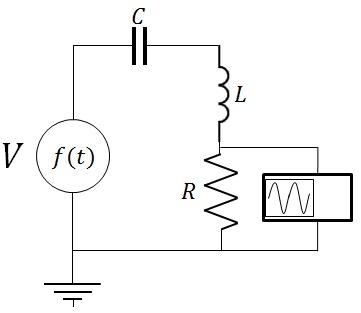
\includegraphics[scale=.7]{RLC-espectro}
\caption{Circuito RLC utilizado para obtener el espectro de frecuencia de Fourier}
\label{fig:RLC-espectro}
\end{figure}

El análisis se realizó para señales $f(t)$  de forma cuadrada y parabólica, las cuales tenían una amplitud$(3.90 \pm 0.02)V$ y $(10.0 \pm 0.2)V$ respectivamente. El objetivo fue poder calcular la trasmisión y obtener los coeficientes dados por \eqref{eq:coef_cuad} y \eqref{eq:coef_parab} en cada caso.

Para ello, al tener en cuanta la importancia del ancho de banda del circuito a la hora de filtrar señales, se usó una resistencia $R=(750 \pm 7)\Omega$ y una inductancia $L=(1003 \pm 5)mH$ la cual aportaba una resistencia $R_L = (243 \pm 2)\Omega$; por lo que de \eqref{eq:resonante} se obtiene $\Delta \omega = (994 \pm 14)Hz$.

Ademas, es claro que las frecuencias que se desean filtrar son múltiplos de la frecuencia $f_0 = \frac{1}{2\tau}$ por lo que no dependen de la forma de la señal. Debido a esto, se impusieron a las dos señales una frecuencia $f_0 = (500 \pm 0.05) Hz$ para garantizar la relación $\Delta\omega << \frac{\pi}{\tau}$.

De esta manera, el parámetro $\omega_0$ podía variar únicamente variando la capacitancia $C$.

Sabiendo esto, se determinaban los valores de $C$ para que $\omega_0$ coincidiese con los armónicos de $f_0$. Y así, para cada armónico, poder medir la caída de potencial sobre la resistencia utilizando el osciloscopio. 

Para garantizar que la frecuencia fuera la de resonancia, se hizo un barrido de mediciones en el intervalo de frecuencias  $[440,560] Hz$, con el fin de encontrar un máximo de transmisión.


\subsection{Modulación y filtración}



\begin{figure}[h]
\centering
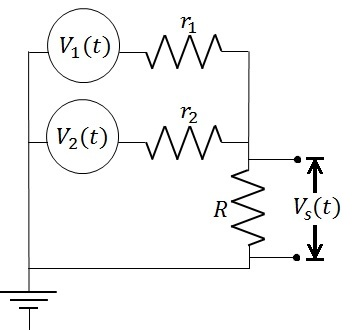
\includegraphics[scale=0.7]{Sumador}
\caption{Sumador}
\label{fig:Sumador}
\end{figure}

\begin{figure}[h]
\centering
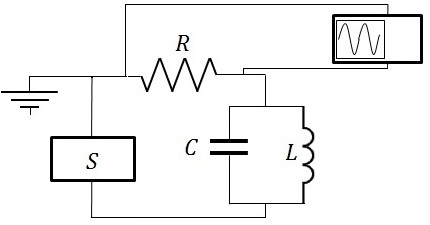
\includegraphics[scale=0.8]{filtro}
\caption{filtro}
\label{fig:filtro}
\end{figure}

%%%%%%%%%%%%%%%%%%%%%%%%%%%%%%%%%%%%%%%%%%%%%%%%%%%%%%%%%%%%%%%%%%%%%%%%%%%%%%%%%%%%%%%%%%%%%%%%%%%%%%%%%%%%%%%%%%%%%%%%%%%%%%%%
% 4.DISCUSIÓN Y RESULTADOS: todo lo que se obtuvo y explicación. Graficos, tablas.
%%%%%%%%%%%%%%%%%%%%%%%%%%%%%%%%%%%%%%%%%%%%%%%%%%%%%%%%%%%%%%%%%%%%%%%%%%%%%%%%%%%%%%%%%%%%%%%%%%%%%%%%%%%%%%%%%%%%%%%%%%%%%%%%

\section{Resultados}
\label{sec:discusion}

\subsection{Analisis de espectro}



\subsection{Modulación y filtración}



%%%%%%%%%%%%%%%%%%%%%%%%%%%%%%%%%%%%%%%%%%%%%%%%%%%%%%%%%%%%%%%%%%%%%%%%%%%%%%%%%%%%%%%%%%%%%%%%%%%%%%%%%%%%%%%%%%%%%%%%%%%%%%%%
%	CONCLUSIONES
%%%%%%%%%%%%%%%%%%%%%%%%%%%%%%%%%%%%%%%%%%%%%%%%%%%%%%%%%%%%%%%%%%%%%%%%%%%%%%%%%%%%%%%%%%%%%%%%%%%%%%%%%%%%%%%%%%%%%%%%%%%%%%%%

\section{Conclusiones}
\label{sec:conclusiones}




%%%%%%%%%%%%%%%%%%%%%%%%%%%%%%%%%%%%%%%%%%%%%%%%%%%%%%%%%%%%%%%%%%%%%%%%%%%%%%%%%%%%%%%%%%%%%%%%%%%%%%%%%%%%%%%%%%%%%%%%%%%%%%%%%
%	APÉNDICE: esas cosas extras que simplemente no tuvieron lo suficiente como para ganarse una sección propia.
%%%%%%%%%%%%%%%%%%%%%%%%%%%%%%%%%%%%%%%%%%%%%%%%%%%%%%%%%%%%%%%%%%%%%%%%%%%%%%%%%%%%%%%%%%%%%%%%%%%%%%%%%%%%%%%%%%%%%%%%%%%%%%%%%



%%%%%%%%%%%%%%%%%%%%%%%%%%%%%%%%%%%%%%%%%%%%%%%%%%%%%%%%%%%%%%%%%%%%%%%%%%%%%%%%%%%%%%%%%%%%%%%%%%%%%%%%%%%%%%%%%%%%%%%%%%%%%%%%%
%	REFERENCIAS: libros, libros, libros.
%%%%%%%%%%%%%%%%%%%%%%%%%%%%%%%%%%%%%%%%%%%%%%%%%%%%%%%%%%%%%%%%%%%%%%%%%%%%%%%%%%%%%%%%%%%%%%%%%%%%%%%%%%%%%%%%%%%%%%%%%%%%%%%%%

%Ejemplo:
\begin{thebibliography}{1}
 \bibitem{Berkeley} Frank S. Crawford, \textit{Berkeley physics course 3: Ondas}, 1994, Editorial Reverte S.A.
\end{thebibliography}
%Para citar: blablabla \cite{Baird}
 
\end{document}





